\documentclass[tikz,border=12pt]{standalone}
\usepackage[T1]{fontenc}
\usepackage{lmodern,amsmath,amssymb}
\usetikzlibrary{arrows.meta,positioning}
\definecolor{ink}{HTML}{183444}
\definecolor{blue}{HTML}{1B6780}
\definecolor{amber}{HTML}{AD601A}
\begin{document}
\hyphenpenalty=10000\exhyphenpenalty=10000
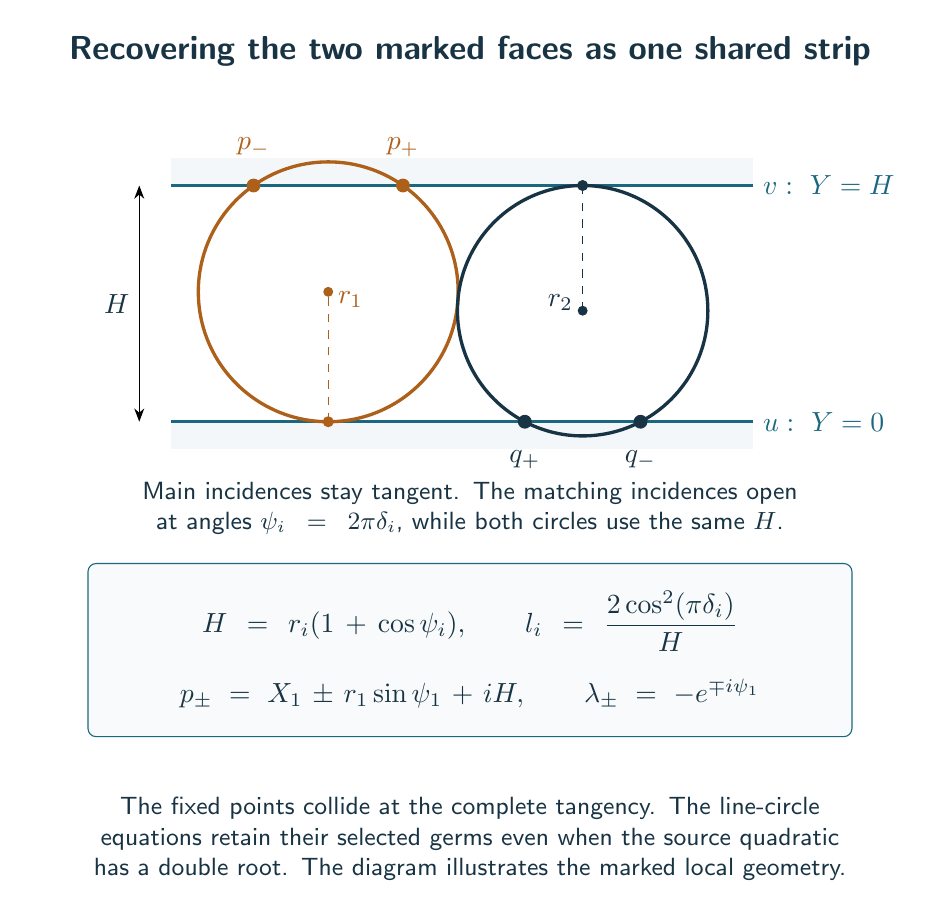
\begin{tikzpicture}[font=\sffamily,text=ink,>=Stealth]
 \node[font=\sffamily\large\bfseries] at (3.6,4.7)
 {Recovering the two marked faces as one shared strip};
 \fill[blue!5] (-.2,-.35) rectangle (7.2,0);
 \fill[blue!5] (-.2,3) rectangle (7.2,3.35);
 \draw[blue,very thick] (-.2,0)--(7.2,0);
 \draw[blue,very thick] (-.2,3)--(7.2,3);
 \node[blue,right] at (7.2,0) {$u:\ Y=0$};
 \node[blue,right] at (7.2,3) {$v:\ Y=H$};
 \draw[<->] (-.6,0)--node[left] {$H$} (-.6,3);

 \pgfmathsetmacro{\ra}{1.65}
 \pgfmathsetmacro{\rb}{1.59}
 \pgfmathsetmacro{\xa}{1.8}
 \pgfmathsetmacro{\xb}{1.8+sqrt(2*3*(\ra+\rb)-9)}
 \pgfmathsetmacro{\pa}{sqrt(\ra*\ra-(3-\ra)*(3-\ra))}
 \pgfmathsetmacro{\pb}{sqrt(\rb*\rb-(3-\rb)*(3-\rb))}
 \draw[amber,very thick] (\xa,\ra) circle (\ra);
 \draw[ink,very thick] (\xb,{3-\rb}) circle (\rb);
 \draw[amber,dashed] (\xa,0)--(\xa,\ra);
 \draw[ink,dashed] (\xb,{3-\rb})--(\xb,3);
 \fill[amber] (\xa,\ra) circle (1.8pt);
 \fill[ink] (\xb,{3-\rb}) circle (1.8pt);
 \node[amber,right] at (\xa,{\ra-.1}) {$r_1$};
 \node[ink,left] at (\xb,{3-\rb+.1}) {$r_2$};
 \fill[amber] (\xa,0) circle (2pt);
 \fill[ink] (\xb,3) circle (2pt);

 \foreach \sgn/\lab in {-1/-,1/+}{
  \fill[amber] ({\xa+\sgn*\pa},3) circle (2.5pt);
  \node[amber,above=7pt] at ({\xa+\sgn*\pa},3) {$p_{\lab}$};
 }
 \foreach \sgn/\lab in {-1/+,1/-}{
  \fill[ink] ({\xb+\sgn*\pb},0) circle (2.5pt);
  \node[ink,below=7pt] at ({\xb+\sgn*\pb},0) {$q_{\lab}$};
 }
 \node[align=center,text width=10.5cm,font=\sffamily\small] at (3.6,-1.1)
 {Main incidences stay tangent. The matching incidences open\\
 at angles $\psi_i=2\pi\delta_i$, while both circles use the same $H$.};

 \node[draw=blue,rounded corners=3pt,fill=blue!3,
       align=center,text width=9cm,inner sep=10pt] at (3.6,-2.9)
 {$H=r_i(1+\cos\psi_i),\qquad l_i=\dfrac{2\cos^2(\pi\delta_i)}{H}$\\[9pt]
 $p_\pm=X_1\pm r_1\sin\psi_1+iH,\qquad
 \lambda_\pm=-e^{\mp i\psi_1}$};
 \node[align=center,text width=11cm,font=\sffamily\small] at (3.6,-5.3)
 {The fixed points collide at the complete tangency. The line-circle\\
 equations retain their selected germs even when the source quadratic\\
 has a double root. The diagram illustrates the marked local geometry.};
\end{tikzpicture}
\end{document}
